\section{Overview}
This chapter outlines the systematic methodology employed to design, develop, and evaluate a web-based restaurant management application. The application leverages modern web technologies, including a React.js frontend \cite{15}, to enhance the dining experience by enabling customers to place orders using QR codes, receive personalized menu recommendations, and choose flexible bill-sharing options. The development process is guided by user-centered design principles, aiming to improve customer satisfaction and operational efficiency for restaurants.

\section{System Design}
The web application is built using React.js \cite{15}frontend with Django backend \cite{16}, with a SQLite database \cite{17}. The frontend is responsible for rendering the user interface and handling user interactions, while the backend manages the business logic and data storage. The frontend and backend communicate via Djano RESTful APIs \cite{15}using Axios \cite{18} from React. The application can hosted on a cloud platform, such as AWS \cite{23} or Heroku \cite{24} or Railway \cite{25}.


\subsection{Backend Architecture}
The backend architecture of the restaurant management system leverages Django's core components. Django was chosen as the backend framework due to its built in features, including the Django ORM for database management, Django REST Framework for API development allows for further scalability, and built-in user authentication and authorization mechanisms. Django models define the database schema, representing core entities like Place, Category, MenuItem, and Order. Views handle the application's business logic, receiving and responding to web requests, interacting with models, and returning JSON responses for use by a React frontend \cite{18}. Django's URL routing directs incoming requests to the appropriate view. The Django REST Framework (DRF) is used to construct a RESTful API for the React interface, providing serializers for complex data to JSON conversion and viewsets for common API operations \cite{20}. Authentication and authorization are handled through Django's built-in system and DRF's mechanisms, such as token authentication. Finally, a database like SQLite is used to persist the system's data \cite{17}.

\subsection{Frontend Architecture}
The frontend architecture of the application leverages React.js to build its user interface, utilizing React components for crafting reusable UI elements like buttons, forms, and menus \cite{15}. State management is handled through React's state and context API, which manage crucial application states, including user authentication, order details, and session information \cite{19}. For navigating between different views without refreshing the page, React Router is employed for client-side routing \cite{22}. The integration with the backend is facilitated through Axios, which is used for making HTTP requests to the Django backend, thereby enabling data exchange between the frontend and the server. The user interface is designed with responsiveness and user-friendliness in mind, aiming to provide an intuitive and visually appealing experience for users. Additionally, Bulma SCSS components are utilized alongside React Components to ensure responsive and uniform styling across the application \cite{22}.

\section{Database Architecture}
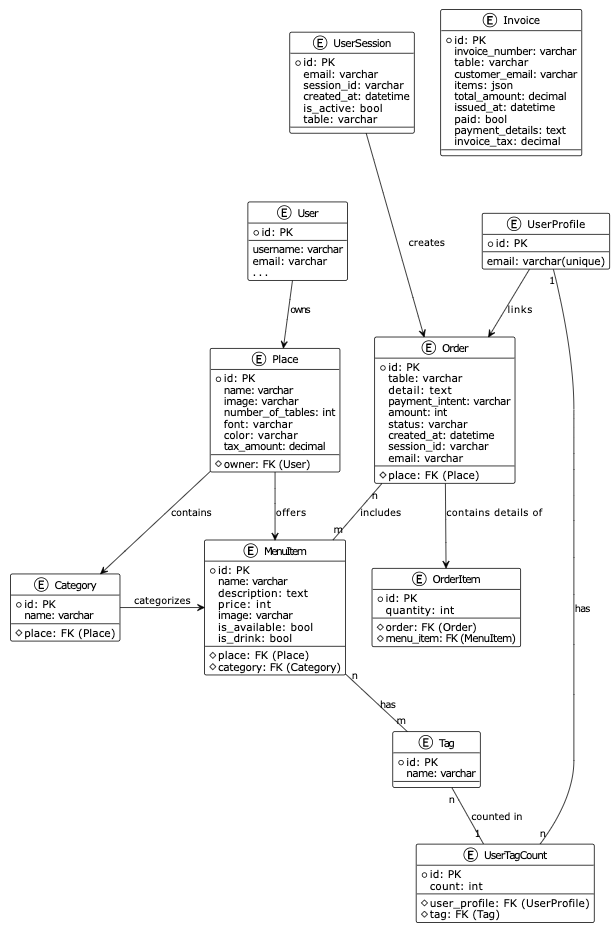
\includegraphics[width=1\textwidth]{images/databasediagram.png}

\subsection{Place}
Represents a restaurant or place that uses the app. It includes details like the owner (linked to the Django \texttt{User} model), name, image, number of tables, and aesthetic customizations (font and color). A new field, \texttt{tax\_amount}, has been added to manage tax calculations.

\subsection{Category}
Organizes menu items into categories (e.g., appetizers, entrees, desserts) for each place. This helps in structuring the menu for easier navigation by the customers.

\subsection{MenuItem}
Details about each menu item, including the place it belongs to, its category, name, description, price, and availability. It also specifies whether the item is a drink and allows for tagging (e.g., vegan, spicy) through a many-to-many relationship with the \texttt{Tag} model.

\subsection{Tag}
Used to label menu items with specific attributes, enhancing the ability to offer personalized recommendations based on customer preferences. Tags are used to describe attributes of food and based on (research) it has been shown that using attributes of food is a good way to recommend food items to customers.

\subsection{UserSession}
Tracks active sessions by customers, including their email, session ID, and table number. It supports functionalities like order tracking and session management. 

\subsection{Order}
Records details of customer orders, including the items ordered (linked through \texttt{OrderItem}), the table and place, payment information, and status. It also tracks the session and customer email.

\subsection{OrderItem}
A through model for the many-to-many relationship between \texttt{Order} and \texttt{MenuItem}, capturing the quantity of each menu item ordered.

\subsection{Invoice}
Manages billing information, including the items ordered, total amount, and payment status. It introduces the \texttt{items} field as a JSON structure to store ordered items, allowing for flexible representation of order details.

\subsection{UserProfile}
Represents a user's profile with a unique email. It is linked to \texttt{Tag} through \texttt{UserTagCount} to track preference metrics.

\subsection{UserTagCount}
Tracks the count of tags associated with a user's orders, facilitating the personalization engine to recommend items based on preferred tags.

\section {Digital Menu Implementation}
QR codes placed on each table serve as the entry point for customers to access the menu and place orders. Upon scanning the QR code with a smartphone, customers are directed to a web interface where they can browse the menu, make selections, and specify their order preferences.
\subsection{Menu Display}
The menu is organized into categories, with each item displaying its name, description, price, and availability. The user interface is designed to be visually appealing and easy to navigate, with a responsive layout that adapts to different screen sizes.
\subsection{Order Placement}
Customers can add items to their order by clicking on the menu items and specifying the quantity. The system tracks the items ordered and the customer's session, allowing for order tracking and billing.
\subsection{Personalized Recommendations}
The application uses the customer's order history and preferences to recommend menu items that match their taste. This is achieved through methods in the \texttt{UserProfile} model, which calculate preferences based on past orders and tag popularity. The algorithm takes into account the most ordered tags and preferred price range to recommend items that align with the customer's preferences.

\section{Recommender Algorithm}
The recommendation algorithm embedded within the \texttt{UserProfile} model of our restaurant management application is designed to offer personalized menu suggestions to users. It analyzes users' past orders, preferences, and price sensitivity to recommend items that align with their tastes.

\subsection{Possible Implementations}
The recommendation algorithm can be implemented in several ways. Here are some of the considered directions.

\subsection*{Collaborative Filtering}
Collaborative filtering recommends items based on the preferences of similar users. It identifies users with similar tastes and suggests items that they have liked. The initial step involves gathering data on customer interactions with the menu. For example, this includes which items customers order, ratings if available, and possibly the context of their orders (time of day, group size, etc). This data is used to identify similarities among users. Then, calculate the similarity between users based on their ordering patterns. Similarity metrics such as Pearson correlation or cosine similarity are used to identify users with similar tastes. The algorithm uses techniques like Singular Value Decomposition (SVD) or Alternating Least Squares (ALS) to analyse datasets. These methods help in predicting a user's interest in an item based on the latent factors extracted from the user-item interaction matrix. Based on the similarity metrics or matrix factorization, generate a list of recommended menu items for each user. This method is effective for discovering new items based on the preferences of a user's peers \cite{26} \cite{27}. However, it requires a large amount of data to generate accurate recommendations.

\subsection*{Content-Based Filtering}
Content-based filtering uses item features to recommend other items similar to what the user likes, based on their previous actions or explicit feedback. In the context of a restaurant application, CBF can personalize menu recommendations by considering the characteristics of menu items (e.g., ingredients, cuisine type, dietary tags) and matching them with a user’s past preferences. The algorithm identifies relevant features of menu items that can influence user preferences, such as type of cuisine, ingredients, dietary restrictions (vegan, gluten-free), spiciness level, and more. These attributes will have to be defined when creating the menu. Use these features to create a profile for each menu item in the database. The algorithm can use a similarity metric (e.g., cosine similarity, Euclidean distance) to compare the feature vectors of the user’s profile with those of each menu item. Calculate a similarity score that indicates how closely an item matches the user's preferences. Rank the menu items based on the similarity score and recommend the top items to the user. This method is effective for providing personalized recommendations based on the attributes of menu items and user preferences \cite{29}.

\subsection*{Hybrid Filtering}
Hybrid Filtering combines collaborative and content-based filtering to leverage the strengths of both approaches. By combining the two methods, the system can provide more accurate and diverse recommendations, addressing the limitations of individual techniques \cite{30}. This method is used by web services such as Netflix and Amazon to provide personalized recommendations to users \cite{33}.

\subsection*{Deep Learning Models}
Neural networks can be used to learn complex patterns in user-item interactions, enabling more accurate and personalized recommendations. These models can capture non-linear relationships between users and items, improving the quality of recommendations. Deep Learning models would need to preprocess the data to convert categorical attributes into numerical or vector representations suitable for neural network input. There are several deep learning architectures that can be used as the recommender algorithm such as Convolutional Neural Networks (CNNs) for analyzing item features or Recurrent Neural Networks (RNNs) and Long Short-Term Memory (LSTM) networks for sequential order data. These models can be trained using backpropagation and optimization techniques like stochastic gradient descent. The model can be evaluated using metrics like Mean Squared Error (MSE) or Mean Absolute Error (MAE) to measure the accuracy of the predictions. This method is effective for capturing complex patterns in user-item interactions and providing accurate recommendations. However, they require large amounts of data and computational resources \cite{31}.

\subsection*{Stable Matching Algorithms}
Stable matching algorithms can be used to match users with items based on their preferences and constraints. By formulating the recommendation problem as a stable matching problem, the system can generate optimal matches between users and items, ensuring fairness and efficiency \cite{32}. Applied to a restaurant usage, this can optimize the recommendation of menu items to customers by aligning diner preferences with menu offerings. The algorithm would need to collect data on user preferences through previous orders, ratings, and explicit feedback. Preferences can include favorite cuisine types, dietary restrictions, and flavor profiles. Then, generate preference lists for both users and menu items. For users, this list ranks menu items based on their historical preferences and feedback. For menu items, create a hypothetical preference list ranking users based on the likelihood of enjoying that item, inferred from user profile similarities and item attributes. Use a stable matching algorithm, like Gale-Shapley, to pair users with menu items. The algorithm iteratively proposes menu items to users based on the preference lists until stable matches are made, where no unmatched pair would both prefer each other over their current matches. After users are recommended items and make selections, collect feedback to refine their preference profiles. This feedback is essential to adjust future recommendations and improve the matching process. However, the need for ongoing user feedback to refine recommendations might increase user interaction requirements, potentially affecting the user experience.

\subsection*{Conclusion}
The approach that has been chosen for this implementation is Hybrid Filtering. The system combines collaborative and content-based filtering to provide more accurate and diverse recommendations. While not using the traditional user-to-user collaborative filtering, the system uses the user's past orders and preferences to recommend items that align with their tastes. This way the customer does not need to provide a preference when they first make their order and the recommender system can instead learn from their past orders. This method leverages the strengths of both collaborative and content-based filtering. The algorithm can use the attributes of menu items and user preferences based of their past orders to recommend items that align with the user's taste profile.


\subsection{User Preferences and Order History Analysis}
The algorithm analyses the user's previous orders to deduce their preferences. The algorithm calculates the average price of the items ordered to establish a preferred price range and identifies the most ordered tags to understand the user's food preferences. This information is then used to score and recommend menu items that align with the user's taste.

\subsection{Tag-Based Recommendations}
The algorithm scores menu items based on the user's preferred tags and price sensitivity. The tags represent the attributes of the items, such as vegetarian, healthy, or spicy. By matching the tags of the menu items with the user's preferred tags, the algorithm can recommend items that are likely to appeal to the user. The reason behind the choice to use tags 

\subsection{Price Sensitivity}
The algorithm calculates the user's preferred price range based on their past orders. By analyzing the average price of the items ordered, the system establishes a price range that the user is comfortable with. This information is used to filter out menu items that fall outside the user's price range, ensuring that the recommendations are tailored to the user's budget. The relationship between price and food choice has been highlighted. Research papers \cite{34} and \cite{35} has indicated that a large percentage of the population prioritizes price as the most determining factor in food choice, often opting for cheaper food regardless of its health or environmental impact.

\subsection{Personalized Recommendations}
The recommendation algorithm scores menu items based on the user's preferred tags and price sensitivity. By matching the tags of the menu items with the user's preferred tags and boosting the score if the price of the food item fits within the user's preferred price range, the algorithm can recommend items that are likely to appeal to the user. The algorithm ranks the menu items based on the score, providing personalized recommendations that align with the user's taste profile. It does the same for both food and drink items

\subsection{Combining Recommendations for Combo Meals}
The recommendation algorithm creates all possible combinations of recommended food and drink items to suggest combo meals to the user. By combining the top recommended food and drink items. This would save the customer time when ordering and would also increase the chances of the customer ordering more items. This is a common strategy used by restaurants to increase sales.

\subsection{Example Usage}
\subsection*{Step 1: Determining the Preferred Price Range}

Assume the user has ordered the following items:

\begin{itemize}
    \item Pizza: \$12 (Quantity: 2)
    \item Burger: \$9 (Quantity: 1)
    \item Salad: \$7 (Quantity: 3)
\end{itemize}

\subsection*{Calculation}

\begin{verbatim}
Total spent on Pizza = $12 * 2 = $24
Total spent on Burger = $9 * 1 = $9
Total spent on Salad = $7 * 3 = $21

Total spent = $24 + $9 + $21 = $54
Total quantity of items ordered = 2 + 1 + 3 = 6

Average price per item = Total spent / Total quantity = $54 / 6 = $9
\end{verbatim}

Preferred price range is calculated as ±20 percent of the average price:
\begin{verbatim}
Lower bound = $9 * 0.8 = $7.20
Upper bound = $9 * 1.2 = $10.80
\end{verbatim}

\subsection*{Step 2: Identifying Most Ordered Tags}

Given tags for each item:
\begin{itemize}
    \item Pizza: ["Italian", "Cheese"]
    \item Burger: ["American", "Beef"]
    \item Salad: ["Vegetarian", "Healthy"]
\end{itemize}

The most ordered tags based on quantity are "Vegetarian" and "Healthy".

\subsection*{Step 3: Scoring and Recommending Menu Items}

New menu items to recommend:
\begin{itemize}
    \item Spaghetti: \$8 ["Italian", "Vegetarian"]
    \item Chicken Wrap: \$10 ["Healthy", "Chicken"]
    \item Fish Tacos: \$11 ["Seafood"]
    \item Veggie Burger: \$9 ["Vegetarian", "American"]
\end{itemize}

\subsection*{Scoring}

Spaghetti scores high for matching "Vegetarian" and being within the price range.
Chicken Wrap scores for "Healthy" and being within the price range.
Fish Tacos score lower due to being outside the price range and no matching tags.
Veggie Burger scores for "Vegetarian" and being within the price range.


\subsection*{Results}

Based on the scoring, the recommended items in order are:
\begin{enumerate}
    \item Spaghetti
    \item Chicken Wrap
    \item Veggie Burger
\end{enumerate}

\section{Flexible Bill Sharing}

This section outlines the systematic steps taken to design, implement, and evaluate this bill splitting implementation.

\subsection{Design Considerations}
A primary focus was to ensure an intuitive and hassle-free interaction with the bill-sharing feature, allowing customers to easily choose between individual payments or sharing the bill with others. The feature needed to accurately calculate and split the bill according to the specific orders and preferences of the diners, providing flexibility in how the bill could be shared. The system has to manage individual and group ordering, allowing customers to order individually or as a group, while ensuring accurate tracking of orders and payments.

\subsection*{Possible Implementations}
There are several ways to implement the bill-sharing feature, each with its own advantages and considerations. Here are some of the possible implementations. One method is to use a session system that allows customers to join a session created by another diner at the same table. This feature is particularly useful for groups who want to combine their orders into a single bill, allowing easy payment splitting without the need for manual calculations or multiple transactions. The system can also provide an option for customers to create individual ordering sessions by entering their email address. This process ensures that each diner's selections are tracked separately, even though they are physically sitting at the same table. At the end of the meal, the group can decide whether to pay separately or together. If they opt for individual payments, each diner pays only for their ordered items. For a shared bill, the total cost is evenly divided among the participants in the joined session, or the payment can be split according to the specific items each person ordered, depending on the application's capabilities and settings. Another possible implementation it to generate new QR codes for each session that is created. This way the system can track the orders and payments. However, this method would require printing a lot of QR codes where as the session system would only require one QR code per table. Hence, the session system is the most sustainable solution over time and it would allow for customer profiling.


\subsection{Implementation}
\begin{itemize}
    \item \textbf{Order Placement via individual Sessions}: When customers scan the QR code at their table, they have the option to create an individual ordering session by entering their email address. This process ensures that each diner's selections are tracked separately, even though they are physically sitting at the same table.
    \item \textbf{Joining Sessions for Shared Billing}: The application provides an option for customers to join a session created by another diner at the same table. This feature is particularly useful for groups who want to combine their orders into a single bill, allowing easy payment splitting without the need for manual calculations or multiple transactions.
    \item \textbf{Separate Payments or Single Payment}: At the end of the meal, the group can decide whether to pay separately or together. If they opt for individual payments, each diner pays only for their ordered items. For a shared bill, the total cost is evenly divided among the participants in the joined session, or the payment can be split according to the specific items each person ordered, depending on the application's capabilities and settings.
\end{itemize}

\section{Admin Panel}
\subsection{Features}
\begin{itemize}
    \item \textbf{Order Tracking}: Provides real-time tracking of customer orders, allowing staff to monitor and manage orders efficiently. This feature allows the adminstrator to keep track of which tables are occupied, the time since the last order, and the status of each order.
    \item \textbf{Billing and Invoice Management}: The adminstrator can manage billing and invoices, for each table and would be able to see all the separate sessions that are on that table. This feature also allows the adminstrator to view and manage the billing and invoices for each table, including the ability to split bills and track payments. All paid and unpaid invoices are stored, allowing the adminstrator to view and manage them as needed. The invoices are designed to work with carbon printers as well.
    \item \textbf{Sales Analysis}: The adminstrator can view sales data such as daily, weekly and monthly sales. The adminstrator can also view the most popular items and the least popular items. This feature also displays the peak hours of the day which along side with the popular items can be used to make decisions on inventory.
    \item \textbf{Global Settings}: The adminstrator can manage global settings such as tax rates, menu themes and fonts. They can also change the name of the restaurant and the logo.
\end{itemize}

\section{Kitchen Display System}
\subsection{Features}
\begin{itemize}
    \item \textbf{Real-time Order Display}: The kitchen display system provides a real-time display of incoming orders, allowing kitchen staff to prepare and manage orders. This feature allows the kitchen staff to view the orders as they come in, and mark them as in progress or completed.
    \item \textbf{Separate Displays}: The system can display orders for different stations on separate screens, allowing staff to focus on their specific tasks. This feature allows the kitchen staff to view the orders that are relevant to their station, and manage them accordingly. Such as the bar which would only display drink orders.
    \item \textbf{Time Warnings:} When the order time exceeds 15 minutes, the order would turn yellow and when it exceeds 25 minutes, the order would turn red. This feature allows the kitchen staff to prioritize orders based on their urgency.
\end{itemize}

\section{Floor Staff Display}
\subsection{Features}
\begin{itemize}
    \item \textbf{Order Tracking}: The orders that have been prepared by the kitchen would be displayed.
    \item \textbf{Table Numbers}: The table numbers of the orders would be displayed.
    \item \textbf{Update Status}: Once the order has been served, the floor staff would be able to update the status of the order as served.
\end{itemize}

\section{Menu Management}
\subsection{Features}
\begin{itemize}
    \item \textbf{Add New Items}: The system should allow restaurant staff to add new items to the menu, including specifying the name, description, price, category, tags which will be used for the recommendation algorithm, and availability of the item. This feature allows the restaurant staff to add new items to the menu as needed, and specify the details of each item.
    \item \textbf{Update Items}: The system should allow restaurant staff to update existing items on the menu, including changing the name, description, price, category, tags, and availability of the item. This feature allows the restaurant staff to update the details of existing items on the menu as needed.
    \item \textbf{Remove Items}: The system should allow restaurant staff to remove items from the menu that are no longer available. This feature allows the restaurant staff to remove items from the menu that are no longer available or have been discontinued.
    \item \textbf{Create Categories}: The system should allow restaurant staff to create new categories for the menu, and assign items to specific categories. This feature allows the restaurant staff to organize the menu into different categories, making it easier for customers to navigate and find items.
    \item \textbf{Manage Tags}: The system should allow restaurant staff to manage tags for each item, specifying the attributes of the item such as vegan, spicy, or gluten-free. This feature allows the restaurant staff to tag items with specific attributes, which will be used for the recommendation algorithm.
\end{itemize}